\documentclass[11pt,a4paper]{article}
\usepackage[margin=2.2cm]{geometry}
\usepackage{graphicx,booktabs,xcolor,array,float}
\usepackage[hidelinks]{hyperref}
\usepackage{fancyhdr}
\pagestyle{fancy}\fancyhf{}
\lhead{34870 Loudspeaker project -- listening test 2, 26 Nov 2026}\rhead{Group 10, System D}\cfoot{\thepage}
\setlength{\parskip}{4pt}\setlength{\parindent}{0pt}
\newcommand{\prov}{\textcolor{red!70!black}{\textbf{[provisional]}}}
\begin{document}

{\LARGE\bfseries Listening test 2, 26 November: results}\\[2pt]
{\large 34870 Electroacoustics, loudspeaker project, Group 10 (System D), IEC listening room}\\[2pt]
{\small Data: \texttt{listening\_results\_2026-11-26.csv} in this folder (the \texttt{/results.csv} export of the
phone form, rows dated 2026-11-26 only, blind conditions filled in). Numbers and figures:
\texttt{python3 analyze\_listening.py} $\rightarrow$ \texttt{numbers.txt}, \texttt{fig\_*.png};
\texttt{estimate\_settings.py} $\rightarrow$ \texttt{est\_numbers.txt}, \texttt{fig\_est\_*.png} (needs scipy).
Test 1 (18 Nov): \texttt{../results\_2026-11-18/}.}

\section*{In one paragraph}
Three listeners (one of them a group member) rated System D as designed (MiniDSP Out~1 $-5.8$\,dB, Rp
8.2\,$\Omega$) at \textbf{8.58 out of 10} overall, against 7.75 in test~1. Every Part~A attribute moved up,
most of all \textbf{treble smoothness} (3.25 $\rightarrow$ 4.17), the weak point of test~1; on the two vocal
tracks it went from 2.50 to 4.17. Bass amount leaned slightly to too little ($-0.25$; $-0.50$ without the
group member). In Part~B the listeners did \textbf{not} follow the woofer gain as test~1 did: bass amount is
$-0.67 / -0.50 / -0.33$ for L / D / H, nearly flat and on the ``too little'' side, and H ($-3.8$\,dB) scored
highest overall. Part~C (tweeter) is \prov: track~4 failed to play five times during the run, and its
ratings contradict the physics (the lower tweeter was called \emph{too much} treble), so it is not used for
conclusions until it is known which samples were affected. With three listeners per test and one session
each, these are trends, not significant results.

\begin{center}\small
\begin{tabular}{@{}>{\raggedright}p{5.0cm}>{\raggedright}p{3.6cm}>{\raggedright}p{3.6cm}>{\raggedright\arraybackslash}p{3.0cm}@{}}\toprule
Question & Test 1, 18 Nov & Test 2, 26 Nov & Reading\\\midrule
Overall, as designed (Part A) & 7.75 (sd 1.71) & 8.58 (sd 0.79) & good, both\\
Bass amount (Part A) & 0.00 & $-0.25$ & about right\\
Treble smoothness (Part A) & 3.25, lowest & 4.17 & no longer a weak point\\
Bass amount L / D / H (Part B) & $-0.33 / +0.17 / +1.33$ & $-0.67 / -0.50 / -0.33$ & test 2 flat\\
Best sample (Part B) & D 2, L 1 & D 2, no diff.\ 1 & D both times\\
Tweeter (Part C), preferred & Rp 3.3: 2, none: 1 & Rp 3.3: 3 \prov & see section 4\\\bottomrule
\end{tabular}
\end{center}

\section*{1\quad The test}
\textbf{Listeners.} Three, all in session 2 (order row 2), one per seat, submitted 13:16--13:17 local time
(12:16--12:17 UTC). Left and right: not group members, no listening-test experience. Middle: \textbf{a group
member} with music experience; the operator sheet says to analyse group members separately, so Part~A is also
given without them. Nobody reported a hearing problem.

\textbf{Parts and tracks.} As in test~1: A (as designed, four tracks: 1 Alison Krauss, 2 Stevie Wonder
\emph{Superstition}, 3 The Prodigy, 4 Pink Floyd); B (woofer at L $-7.8$, D $-5.8$ twice, H $-3.8$\,dB,
tracks 2 then 3); C (Rp 8.2 against 3.3\,$\Omega$, tracks 4 then 2). Track~2 was still \emph{Superstition}
in test~2; it is replaced by Sade, \emph{Smooth Operator} from now on (not used in tests 1 or 2).
Playback: Spotify through the control panel on the laptop, Schiit Modi, MiniDSP.

\textbf{Order.} Session 2 = order row 2: Part B samples H, D, L, D; Part C sample X = Rp 3.3\,$\Omega$,
Y = Rp 8.2\,$\Omega$ (test~1 had the opposite Part~C order).

\textbf{Deviations.} Track~4 (\emph{Shine On You Crazy Diamond}) failed to start five times
(12:52, 13:09 twice, 13:10, 13:13): Spotify jumped forward to about 5:20 after loading it, the panel did not
correct a forward jump, so the track stayed silent and stopped. The panel has been fixed since. All five
failures fall inside this one session, which ran about 12:25--13:15. The woofer level during Part~C was not
noted; the sheet says to set Out~1 back to $-5.8$\,dB after Part~B, and Part~B ended on D ($-5.8$\,dB) in
this order anyway, so the estimates below assume $-5.8$\,dB.

\section*{2\quad Part A: the loudspeaker as designed}
\begin{figure}[H]\centering
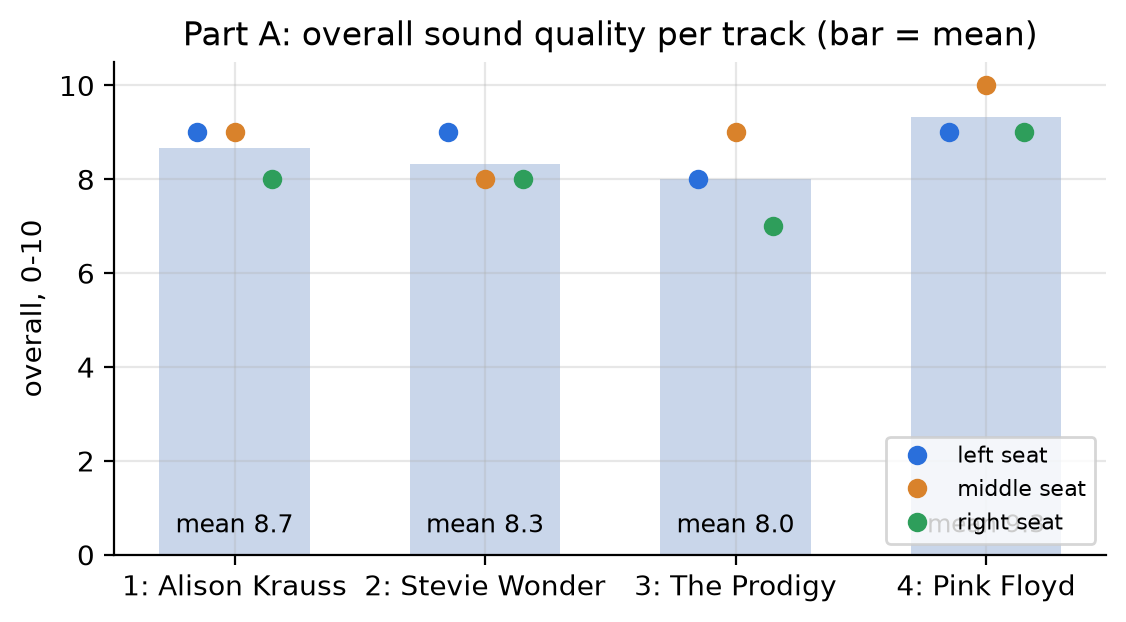
\includegraphics[width=0.78\linewidth]{fig_A_overall.png}\\[2pt]
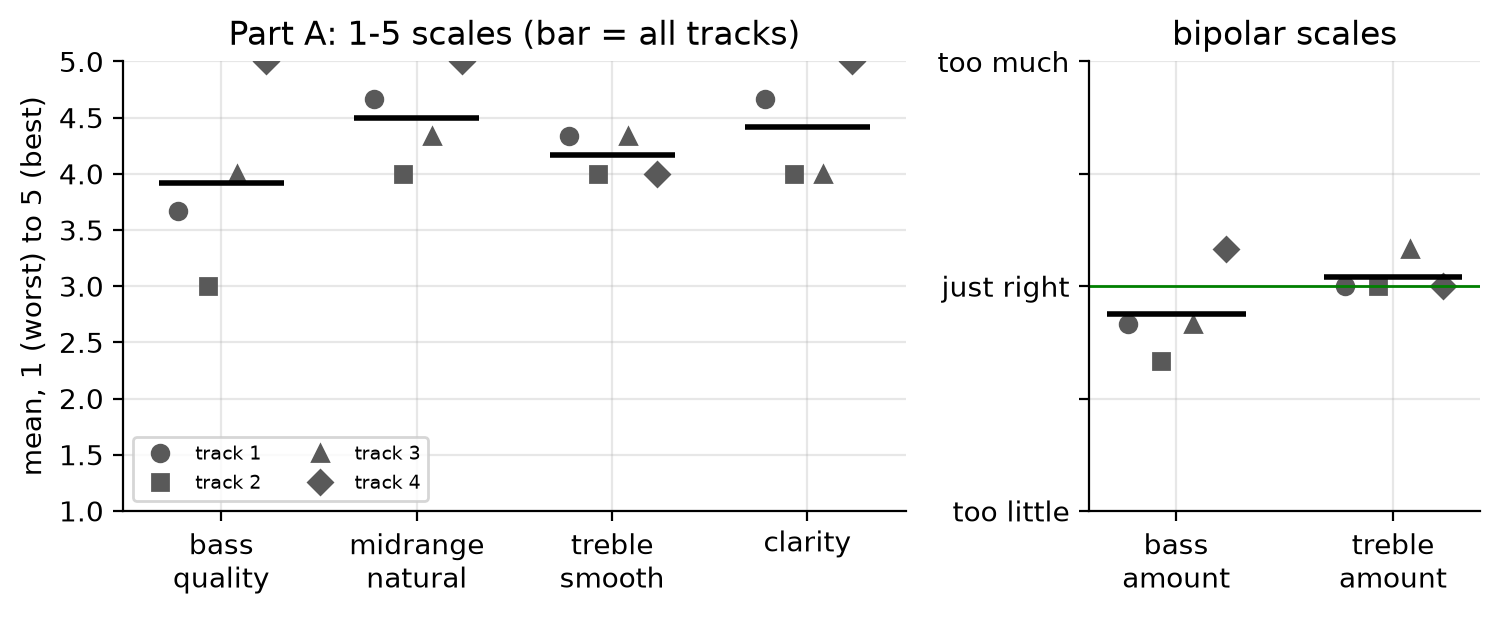
\includegraphics[width=0.95\linewidth]{fig_A_profile.png}
\caption{Top: overall per track, each dot one listener. Bottom: mean per track (markers) and over all tracks
(bars). The green line is ``just right''.}
\end{figure}

\begin{center}\small
\begin{tabular}{@{}lcccccc@{}}\toprule
Attribute & Track 1 & Track 2 & Track 3 & Track 4 & All & Test 1, all\\\midrule
Bass amount ($-2\ldots+2$) & $-0.33$ & $-0.67$ & $-0.33$ & $+0.33$ & $-0.25$ & $0.00$\\
Bass quality (1--5) & 3.67 & 3.00 & 4.00 & 5.00 & 3.92 & 3.67\\
Midrange natural (1--5) & 4.67 & 4.00 & 4.33 & 5.00 & 4.50 & 3.83\\
Treble amount ($-2\ldots+2$) & $0.00$ & $0.00$ & $+0.33$ & $0.00$ & $+0.08$ & $+0.33$\\
Treble smoothness (1--5) & 4.33 & 4.00 & 4.33 & 4.00 & \textbf{4.17} & 3.25\\
Clarity (1--5) & 4.67 & 4.00 & 4.00 & 5.00 & 4.42 & 3.75\\
Overall (0--10) & 8.67 & 8.33 & 8.00 & 9.33 & \textbf{8.58} & 7.75\\\bottomrule
\end{tabular}
\end{center}

The balance is close to neutral: treble amount $+0.08$ and bass amount $-0.25$. Unlike test~1 there is no
weak attribute; the lowest is bass quality on track~2 (3.00, the same as in test~1). Without the group member
(two listeners, 8 ratings each): overall 8.38, treble smoothness 4.00, bass amount $-0.50$, so the picture
does not depend on him. The left listener rated bass amount $-1$ on every track and wrote ``the bass volume
was consistently too low \dots\ you could only hear it, not feel it''.

\textbf{By seat:} overall left 8.75, middle 9.00, right 8.00; treble amount left $0.00$, middle $0.00$,
right $+0.25$. In test~1 the left seat was lowest (6.25) and heard the most treble; here it does not stand
out, so the test-1 seat effect was most likely that listener, not the seat. Track~4 in Part~A may also have
been affected by the playback failures (see section 9).

\section*{3\quad Part B: woofer level}
\begin{figure}[H]\centering
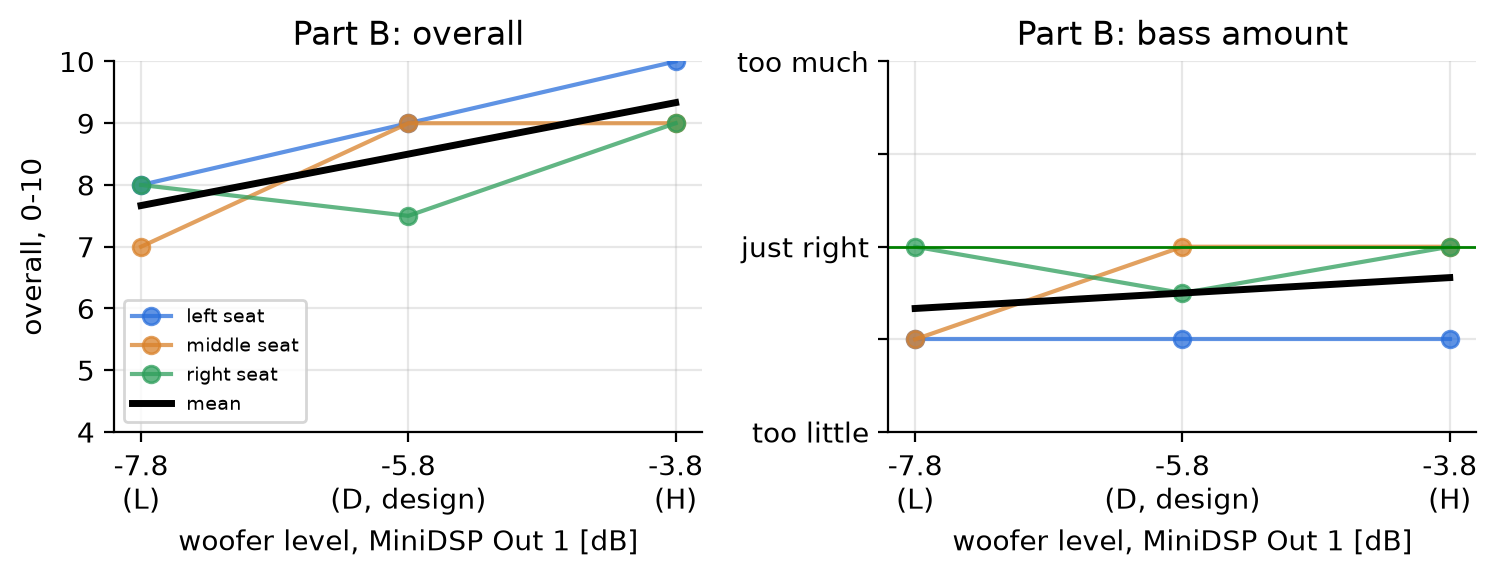
\includegraphics[width=0.95\linewidth]{fig_B_woofer.png}
\caption{Overall and bass amount against the MiniDSP Out~1 gain. Thin lines: listeners (D is the mean of its
two plays); thick line: mean.}
\end{figure}

\begin{center}\small\setlength{\tabcolsep}{4pt}
\begin{tabular}{@{}lcccccc@{}}\toprule
 & & \multicolumn{2}{c}{Test 2} & \multicolumn{2}{c}{Test 1} & \\
Condition & Out 1 gain & Overall & Bass amount & Overall & Bass amount & Best (t1 / t2)\\\midrule
L & $-7.8$\,dB & 7.67 & $-0.67$ & 8.67 & $-0.33$ & 1 / 0\\
D (design, twice) & $-5.8$\,dB & 8.50 & $-0.50$ & 7.67 & $+0.17$ & 2 / 2\\
H & $-3.8$\,dB & 9.33 & $-0.33$ & 7.67 & $+1.33$ & 0 / 0\\\bottomrule
\end{tabular}\\[2pt]
{\footnotesize Test 2: ``no difference'' chosen once (right seat).}
\end{center}

In test~2 the bass-amount ratings barely move with the gain ($-0.67$ to $-0.33$ over 4\,dB) and stay on
the ``too little'' side; overall rises from L to H. The left listener answered $-1$ for all four samples;
the group member wrote that 2\,dB ``doesn't make much of a difference'' and that the bass in
\emph{Superstition} is ``so low, it doesn't make sense to compare it''. The repeat of D: 10/8, 9/9, 7/8
(differences 2, 0, 1), as consistent as in test~1. Both tests chose D as best sample twice.

\textbf{Reading across both tests:} test~1 heard H as clearly too much bass, test~2 heard all three as
slightly too little. Pooled (6 listeners), bass amount is $-0.50 / -0.17 / +0.50$ for L / D / H: the design
level D is still the one nearest ``just right''. The disagreement between the sessions, and the comment on
track~2, support replacing \emph{Superstition} with a track with more bass before a third test. Raising the
woofer by 2\,dB is not ruled out by test~2 (H scored best) but was rejected by test~1.

\section*{4\quad Part C: tweeter level \prov}
\begin{figure}[H]\centering
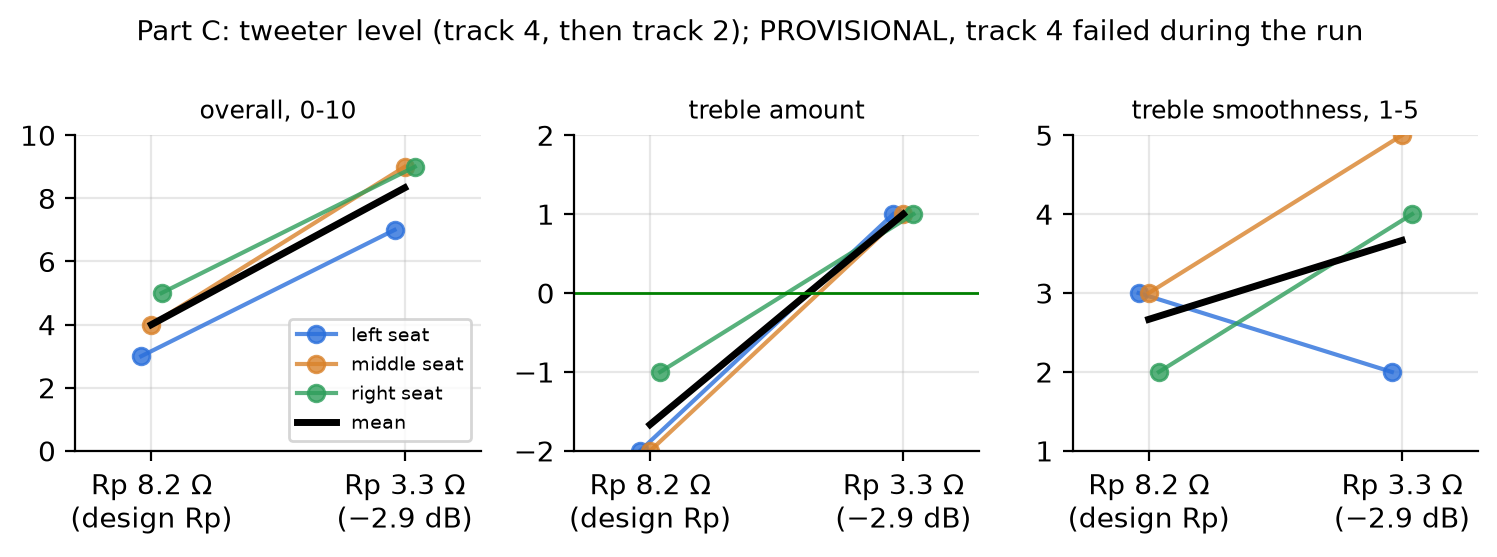
\includegraphics[width=0.95\linewidth]{fig_C_tweeter.png}
\caption{Each listener's two samples joined by a line; thick line: mean. In this session Rp 3.3\,$\Omega$
was played first (X), Rp 8.2\,$\Omega$ second (Y). Provisional: see the text.}
\end{figure}

\begin{center}\small
\begin{tabular}{@{}lccccc@{}}\toprule
Condition & Played & Overall (0--10) & Treble amount & Smoothness (1--5) & Preferred\\\midrule
Rp 8.2\,$\Omega$ (design) & Y, second & 4.00 (sd 1.00) & $-1.67$ & 2.67 & 0\\
Rp 3.3\,$\Omega$ (tweeter $-2.9$\,dB) & X, first & 8.33 (sd 1.15) & $+1.00$ & 3.67 & 3\\\bottomrule
\end{tabular}
\end{center}

All three preferred Rp 3.3\,$\Omega$, and in test~1 it was preferred 2 to 0 while being played second, so the
preference is not simply an order effect. But \textbf{two things make this part unreliable as it stands}:
\begin{enumerate}\setlength{\itemsep}{1pt}
\item \textbf{The treble ratings point the wrong way.} Rp 3.3\,$\Omega$ puts the tweeter 2.9\,dB
\emph{lower}, yet all three called it slightly too much treble ($+1$) and the design value too little
($-2, -2, -1$). In test~1 the direction was as expected ($+0.33 \rightarrow 0.00$). Either the samples did not
contain what the table says (Rp swapped the other way round, or a sample heard with track~2 only, or after
retries), or the listeners compared two different pieces of music.
\item \textbf{Sample Y scored 4.0 overall}, far below anything else in the session (Part~A and B never went
below 7). That looks more like a disturbed sample (silence, restarts, only part of the programme) than a
2.9\,dB tweeter change.
\end{enumerate}
If the Rp values were actually swapped (X = 8.2, Y = 3.3), the treble ratings would make sense and the
preference would flip to the design value. So Part~C of test~2 is \textbf{not used for the design decision}
until the operator confirms which Rp was fitted for X and Y and which samples were hit by the track~4
failures.

\section*{5\quad Estimated responses of the settings that were played}
Built exactly as in test~1 (\texttt{estimate\_settings.py}, from the 12-Nov anechoic runs S\_3 and S\_4,
on axis, 1/6 octave, 0\,dB = the design's median 150\,Hz--15\,kHz). The woofer level in Part~C is assumed
to be $-5.8$\,dB (section 1).

\begin{figure}[H]\centering
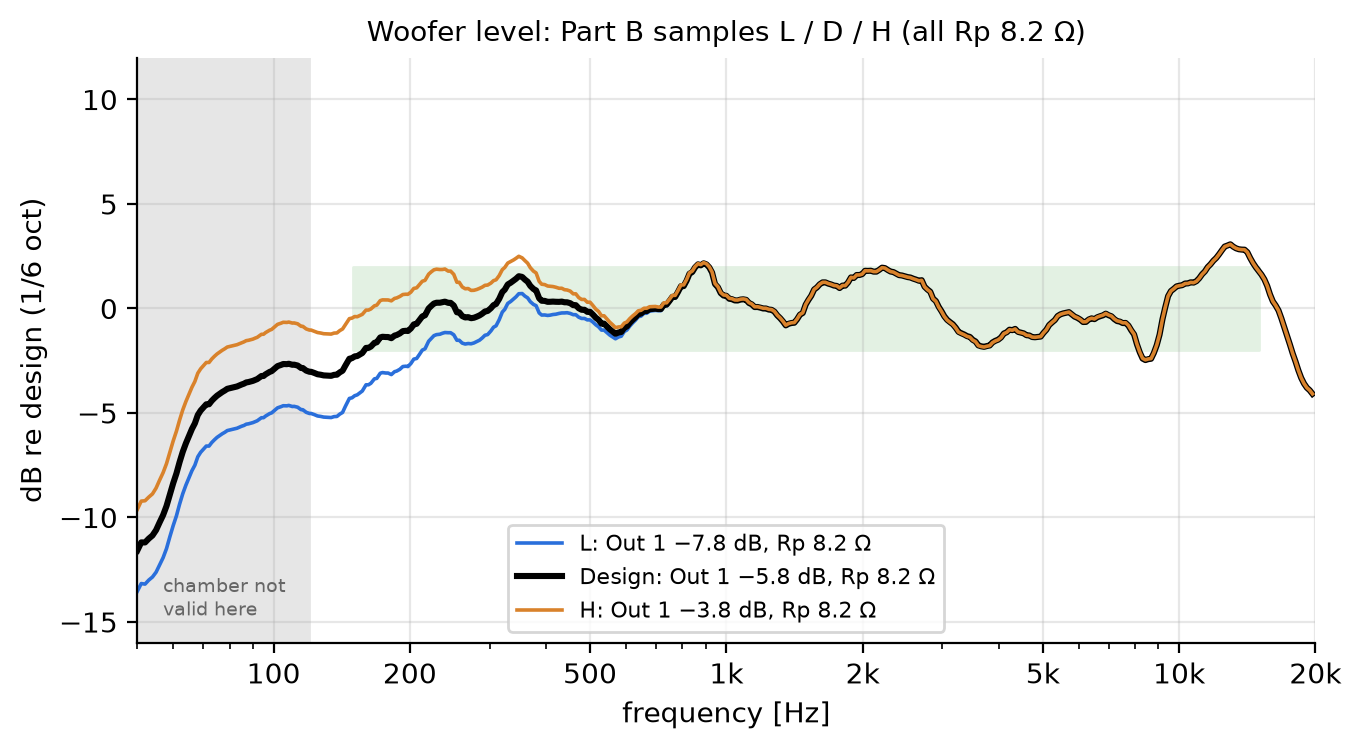
\includegraphics[width=0.92\linewidth]{fig_est_woofer.png}
\caption{Part B samples L, D (design) and H, all with Rp 8.2\,$\Omega$.}
\end{figure}
\begin{figure}[H]\centering
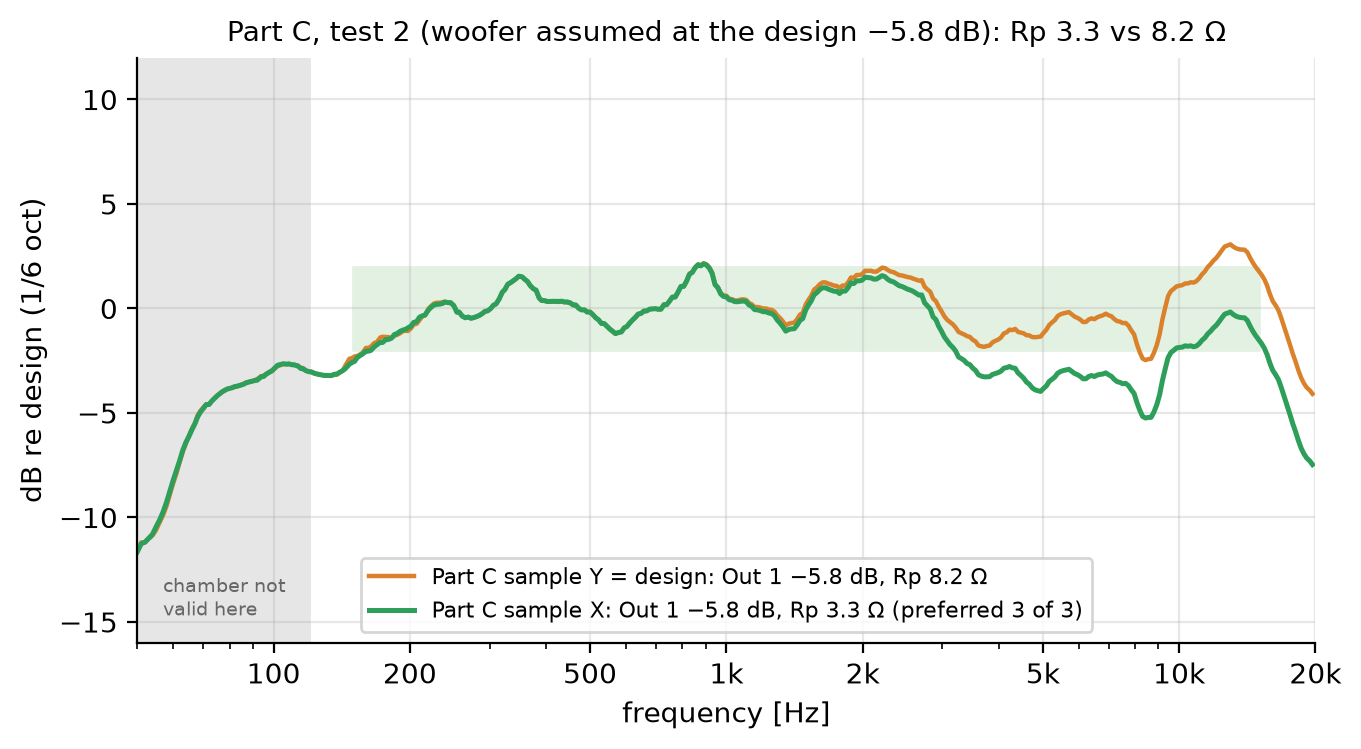
\includegraphics[width=0.92\linewidth]{fig_est_partC.png}
\caption{Part C of test 2 with the woofer assumed at the design $-5.8$\,dB: Rp 8.2\,$\Omega$ (= the design)
against Rp 3.3\,$\Omega$.}
\end{figure}

\begin{center}\small\setlength{\tabcolsep}{3.5pt}
\begin{tabular}{@{}llrrrrrr@{}}\toprule
Setting & Played in (test 2) & 150--300 & 300--500 & 2--4k & 4--8k & 8--15k & spread\\\midrule
Out 1 $-5.8$, Rp 8.2 (design) & A, B sample D, C sample Y & $-0.8$ & $+0.1$ & $+0.4$ & $-0.9$ & $+1.1$ & 5.5\\
Out 1 $-7.8$, Rp 8.2 & B sample L & $-2.3$ & $-0.5$ & $+0.4$ & $-0.9$ & $+1.1$ & 7.2\\
Out 1 $-3.8$, Rp 8.2 & B sample H & $+0.6$ & $+0.9$ & $+0.3$ & $-1.0$ & $+1.1$ & 5.5\\
Out 1 $-5.8$, Rp 3.3 & C sample X (woofer assumed) & $-0.6$ & $+0.2$ & $-0.4$ & $-3.4$ & $-1.9$ & 7.4\\
\bottomrule
\end{tabular}\\[2pt]
{\footnotesize Band medians in dB relative to the same curve's 500\,Hz--2\,kHz median; spread = peak-to-peak
150\,Hz--15\,kHz in dB. Part B settings are the same as in test 1.}
\end{center}
At the design woofer level, Rp 3.3\,$\Omega$ again removes the +3\,dB rise near 12--13\,kHz but pulls
4--8\,kHz down by a further 2.5\,dB (spread 5.5 $\rightarrow$ 7.4\,dB), the same trade-off as in test~1.

\section*{6\quad Test 1 and test 2 compared}
\begin{figure}[H]\centering
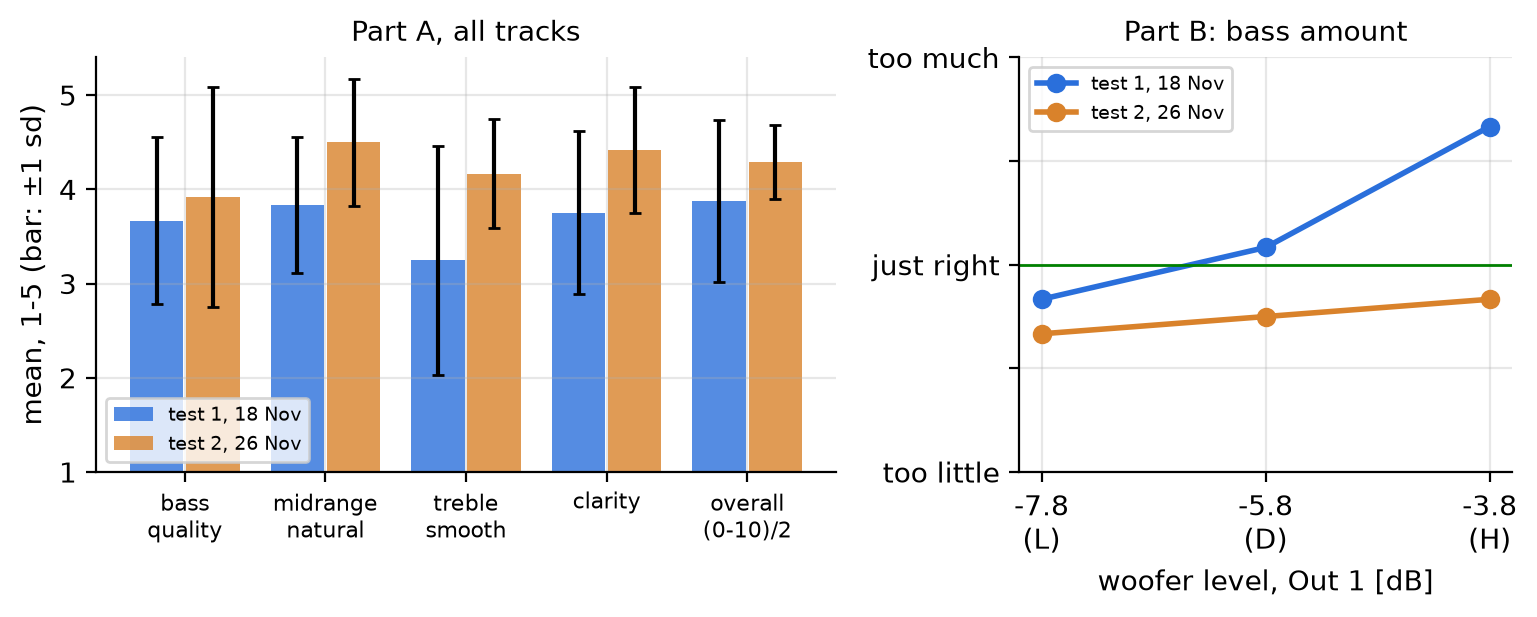
\includegraphics[width=0.95\linewidth]{fig_compare.png}
\caption{Left: Part A means over all tracks (overall halved to fit the 1--5 axis), bars $\pm1$\,sd.
Right: Part B bass amount against woofer gain.}
\end{figure}
\begin{itemize}\setlength{\itemsep}{1pt}
\item \textbf{Same speaker, same tracks, same settings, higher scores.} Part~A overall 7.75 $\rightarrow$
8.58 and every quality attribute up by 0.25--0.92. Pooled over both tests (6 listeners, 24 ratings):
overall 8.17, treble smoothness 3.71, bass amount $-0.12$, treble amount $+0.21$.
\item \textbf{The treble complaint of test~1 did not come back.} Treble smoothness on the vocal tracks:
2.50 $\rightarrow$ 4.17; nobody wrote about harsh treble in test~2. With one session each, a different set of
three listeners is the most likely cause; nothing in the speaker changed.
\item \textbf{Woofer level:} the two sessions disagree on how much bass H has, but both chose D as best
sample twice and pooled D is nearest ``just right''.
\item \textbf{Tweeter:} Rp 3.3\,$\Omega$ preferred in both tests and in both orders, but test~1 was played with
the woofer at $-3.8$\,dB and test~2 is provisional (section 4).
\end{itemize}

\section*{7\quad What the listeners wrote}
\begin{itemize}\setlength{\itemsep}{1pt}
\item Left: ``The bass quality was genuinely good, but it lacked volume'' (Part~A); D ``sounded a bit clearer
in the mid/high ranges''; L ``a bit more muddy, slightly suppressed high/mid ranges''; last question: ``The
bass volume was consistently too low \dots\ you could only hear it, not feel it. For the most part it was
crisp audio.''
\item Middle (group member): ``sometimes a bit boxy, maybe because there is only one speaker''; on Part~B,
\emph{Superstition}'s bass too low to compare, Prodigy good; 2\,dB steps too small; ``idk i love it already''.
\item Right: no comments.
\end{itemize}
(As written; full text in \texttt{numbers.txt}.)

\section*{8\quad Conclusions for the design (Parts A and B only)}
\begin{enumerate}\setlength{\itemsep}{2pt}
\item \textbf{As designed, the speaker is rated good to very good}: 8.58 in test~2, 8.17 over both tests.
\item \textbf{Woofer level: keep $-5.8$\,dB for now.} Pooled over both tests it is nearest ``just right'' and
was chosen best four times. Test~2 leans to slightly more bass; a third test with a bass-rich track~2 (and
perhaps 3\,dB steps instead of 2\,dB) would settle it.
\item \textbf{Treble:} test~2 does not confirm the treble problem of test~1. Whether to change Rp waits for
the Part~C questions to be answered.
\end{enumerate}

\section*{9\quad Limits}
Three listeners in one session per test, one of them a group member in test~2; one listener per seat; one
fixed order per test. The track~4 failures may also have touched Part~A track~4 (rated highest, 9.33) if a
retry was needed there. Part~C of test~2 is provisional (section 4). No test of significance is meaningful
at $n=3$ per test.

\end{document}
